%!TEX root = ../main.tex
%%%%%%%%%%%%%%%%%%%%%%%%%%%%%%%%%%
% Links:
%
% Difficulty:
% Companies: 
%%%%%%%%%%%%%%%%%%%%%%%%%%%%%%%%%%


%\begin{figure}
%	\centering
%	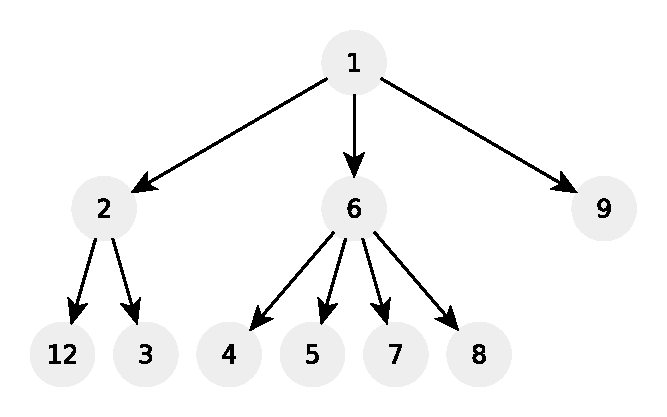
\includegraphics[width=\textwidth]{sources/min_substitution_in_ab_string/images/example1}
%	\caption[Sample short cpation]{Sample Caption}.
%	\label{fig:min_substitution_in_ab_string:example1}
%\end{figure}

\chapter{TITLE OF THE CHAPTER}
\label{ch:min_substitution_in_ab_string}
\section*{Introduction}

\section{Problem statement}
\begin{exercise}
\label{example:min_substitution_in_ab_string:exercice1}
\verbatim{You are given a string S of length N consisting of characters 'a' and 'b' with additional empty gaps represented by '?'. Your task is to replace every such gap with either an 'a' character or a 'b' character so that the longest fragment of S, consisting only of 'a' characters or 'b' characters, is as short as possible.

For example, for S = "aa??bbb", if you replace "??" with "aa", the longest fragment consisting of equal characters will have length 4: "aaaabbb". You can obtain a better result by replacing "??" with "ba", resulting in "aababbb". Then the longest fragment consisting of equal characters will have length 3.

Write a function:

int solution(string &S);

that, given a string S of length N, returns the minimum possible length of the longest fragment of S consisting of equal characters after replacing all "?" characters with letters.

Examples:

1. Given S = "aa??bbb", your function should return 3, as explained above.

2. Given S = "a?b?aa?b?a", your function should return 2. Question marks can be replaced in the following way: "aabbaabbaa".

3. Given S = "??b??", your function should return 1.

4. Given S = "aa?b?aa", your function should return 3.

Write an efficient algorithm for the following assumptions:

string S consists only of the following characters: "a", "b" and/or "?";
N is an integer within the range [1..100,000].
}
	%example1
	\begin{example}
		\label{example:min_substitution_in_ab_string:example1}
		\hfill \
	}
		
	\end{example}

	%example2
	\begin{example}
		\label{example:min_substitution_in_ab_string:example2}
		\hfill \
		
	\end{example}

	\begin{example}
		\hfill \
	
	\label{ex:min_substitution_in_ab_string:example3}
	\end{example}

	\begin{example}
		\hfill \

	\label{ex:min_substitution_in_ab_string:example4}	
	\end{example}
\end{exercise}

\section{Clarification Questions}

\begin{QandA}
	\item 
	\begin{answered}
		\textit{}
	\end{answered}
	
\end{QandA}

\section{Discussion}
\label{min_substitution_in_ab_string:sec:discussion}


\subsection{Brute-force}
\label{min_substitution_in_ab_string:sec:bruteforce}

\begin{minipage}{\linewidth}
	\lstinputlisting[language=c++, caption={Sample Caption},label=list:min_substitution_in_ab_string]{sources/min_substitution_in_ab_string/min_substitution_in_ab_string_solution1.cpp}
\end{minipage}

